\documentclass{article} 
\usepackage{tikz}
\usetikzlibrary{trees}
\usetikzlibrary{arrows}%flechas!!!
\begin{document}

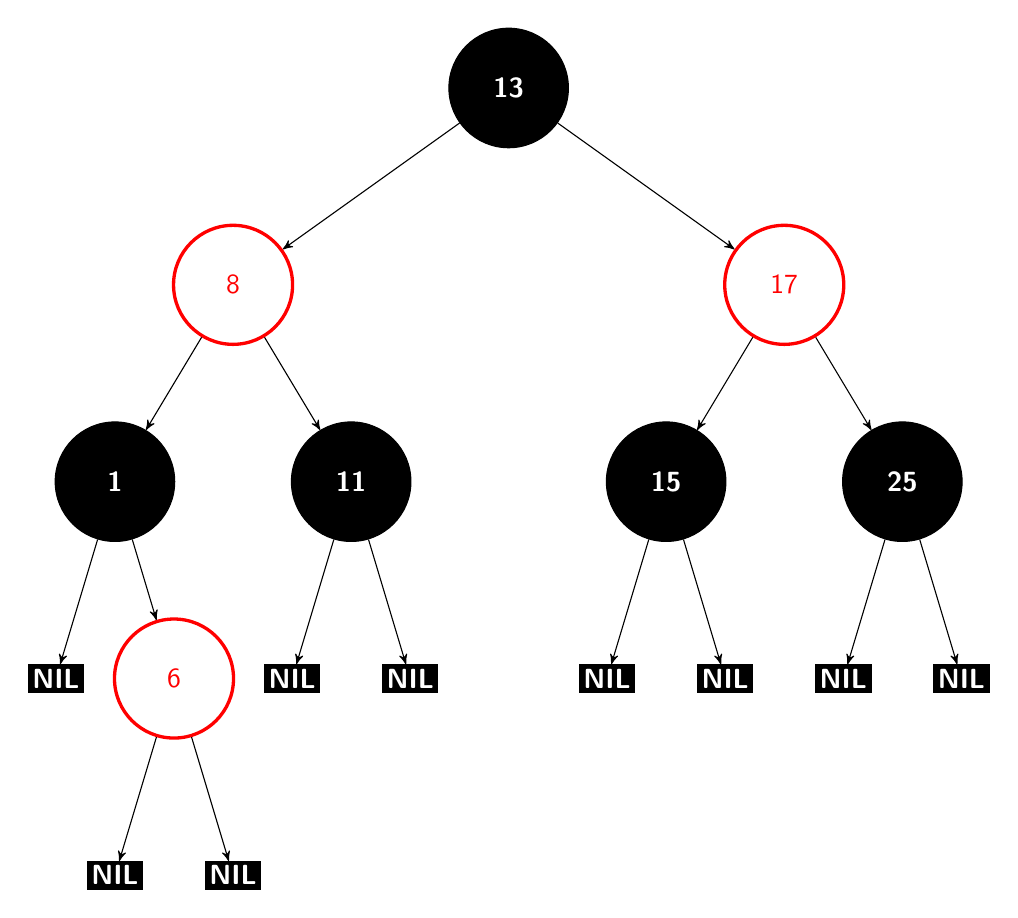
\begin{tikzpicture}[->,>=stealth',
 level 1/.style={sibling distance=7cm},
 level 2/.style={sibling distance=3cm},
 level 3/.style={sibling distance=1.5cm},
 level distance = 2.5cm] 

%Definicion de los nodos, ancho fijo, color fijo, forma, etc.
\tikzset{
  treenode/.style = {align=center, inner sep=0pt, text centered,
    font=\sffamily}, 
  black_node/.style = {treenode, circle, white, font=\sffamily\bfseries, draw=black,
    fill=black, text width=1.5cm},% Nodos negros
  red_node/.style = {treenode, circle, red, draw=red, text width=1.5cm, very thick},% Nodos rojos
  NIL/.style = {treenode, rectangle, white, fill=black,font=\sffamily\bfseries, draw=black, minimum width=2em, minimum height=1em}%NIL
}


  \node [black_node] {13}
    child { node [red_node] {8}
      		child {node [black_node] {1}
			child {node [NIL] {NIL}}
			child {node [red_node] {6}
				child {node [NIL] {NIL}}
				child {node [NIL] {NIL}}}}
      		child {node [black_node] {11}
      			child {node [NIL] {NIL}}
      			child {node [NIL] {NIL}}}
    }
    child {node [red_node] {17}
    		child {node [black_node] {15}
			child {node [NIL] {NIL}}
			child {node [NIL] {NIL}}}
    		child {node [black_node] {25}
			child {node [NIL] {NIL}}
			child {node [NIL] {NIL}}}
    };

\end{tikzpicture}
\end{document}
